Accounting for power and temperature is key to achieving effectiveness,
efficiency, and robustness. However, the power and temperature characteristics
of the system under development are difficult to describe mathematically or
algorithmically. Modern systems are complex, and many aspects are inherently
uncertain to the designer due to such phenomena as process variation
\cite{chandrakasan2000}, aging \cite{coskun2006}, and varying workload.

The above concern is particularly hard to address from a theoretical standpoint;
it can be better dealt with taking a more pragmatic approach, namely, making use
of runtime data. Assuming that the system provides mechanisms for profiling and
monitoring, direct or indirect power and temperature readings are an invaluable
source of information for making proactive power- and temperature-aware
decisions \cite{chaudhry2015, coskun2008}.

Acting proactively requires forecasting the future by learning from the past,
which is typically accomplished by virtue of statistics and adjacent fields such
as machine learning \cite{bishop2006}. In this case, a proactive governor
contains a learning component, which assimilates relevant runtime data and makes
predictions. To give a concrete example, in \cite{coskun2008}, temperature
forecasting is based on an autoregressive moving-average model, enabling the
development of an efficient thermal management strategy for multiprocessor
systems. The work in \cite{kumar2010} aids runtime thermal management by
developing an on-chip temperature predictor based on artificial neural networks.
The analysis and mitigation of the impact of process variation undertaken in
\cite{juan2014} are facilitated by a linear-regression model trained on leakage
measurements in order to predict peak temperatures.

In the above, we have argued for the usage of learning-based techniques for the
management of electronic systems, and we have put emphasis on those techniques
that learn online, that is, at runtime on the chip, as they are capable of
adaptation. However, the present work is not concerned with the development of
any particular technique of this kind. Instead, the goal of our work is to
provide an infrastructure that facilitates the development of such techniques,
and this infrastructure addresses the following major concern.

\begin{figure}
  \centering
  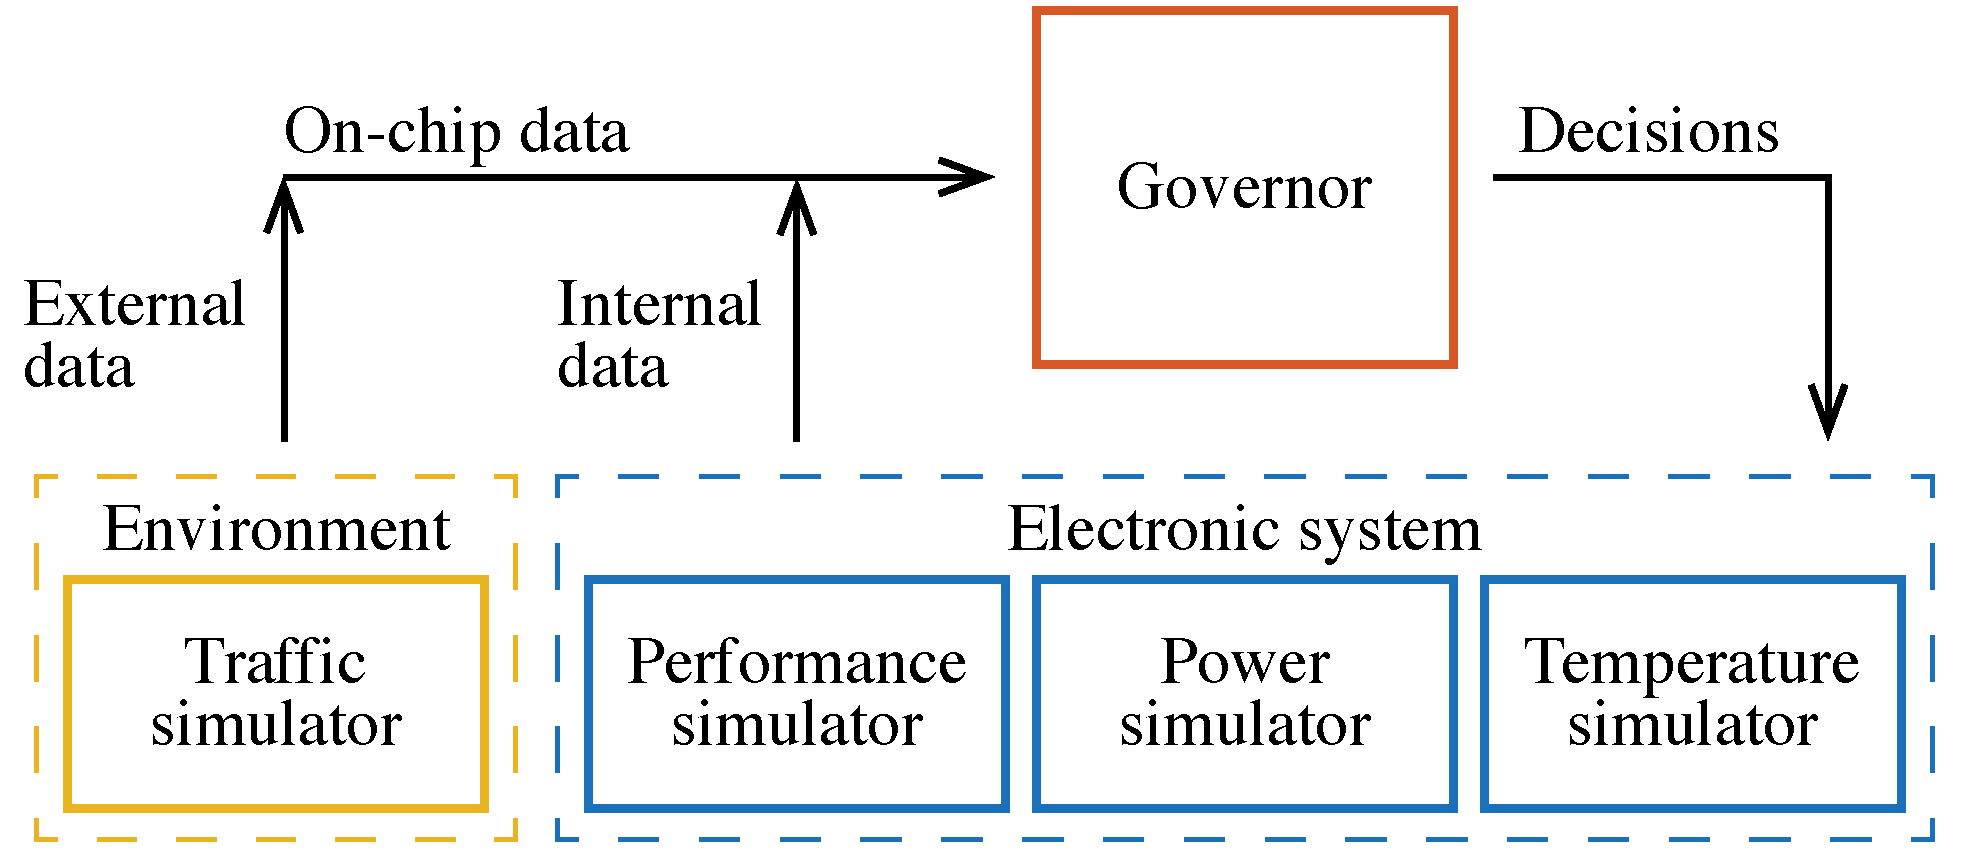
\includegraphics[width=1.0\columnwidth]{include/assets/figures/development.pdf}

  \caption{An experimental setup for developing management strategies
  (governors). \emph{Online data} refers to the data available on the chip
  regardless of their origin. The right dashed box should be understood at a
  single module, and the corresponding arrows should be treated accordingly.}

  \flab{development}
\end{figure}

Regardless of the learning tool utilized, the tool needs data to learn from.
Prior to a physical instantiation of the platform under consideration, all the
hope rests on the shoulders of computer models and simulators. The need for
simulators is not any lower even when an existing platform is concerned. The
platform might not be available to the interested party, or it might not be an
appropriate place for early experimentation and fluid exploration, which is
arguably the most common scenario in research. In such cases, computer
simulators are of great help, and their ubiquitous usage speaks to this
assertion. Therefore, a typical research environment used for developing a
governor of an electronic system is composed of a number of simulators,
providing data to and processing data from the governor. An illustration of such
an environment is given in \fref{development}, which will be discussed further
later on.

Simulations can be undertaken on different levels. In order to be useful for
learning purposes, simulations should be sufficiently detailed so that they
capture well the traits of real systems. Although detailed simulations are
practical for the design of individual components, such simulations fall short
when it comes to complex systems. A modern multiprocessor system is reasonably
complex, and it might take days for a state-of-the-art simulator to simulate a
short, in wall-clock time, program running on such a system. This scheme is not
affordable for designing data-driven techniques as they require many simulations
with potentially large payloads.

The conclusion is that real data are rarely available, and simulation data are
prohibitively time consuming to obtain. Both are severely limiting from the
standpoint of a researcher trying to leverage the rich machinery of statistics
and machine learning. The need for alternative sources of high-quality data is
prominent, and providing such an alternative source is the very goal of this
work. We are to build a highly responsive (time-wise) research infrastructure,
which is supposed to be used for the development of online, data-driven, power-
and temperature-aware solutions for multiprocessor systems instead of the one
depicted in \fref{development}.
